\icode{E-MI-SI-L2-261109-001}
一光滑圆环固定在竖直平面内，其上套有两个小球\(A\)和\(B\)，两球由细绳连接，恰好能在图示位置均保持静止状态。此时，\(B\)球与环的圆心\(O\)点处在同一水平面上，\(A\)、\(B\)间的细绳呈伸直状态，并与水平面成\qty{30}{\degree}角，则可知\(A\)球与\(B\)球的质量之比为\paren[]

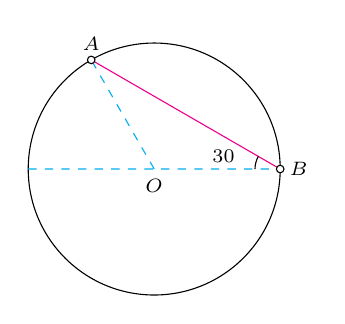
\begin{tikzpicture}[scale=.8,font=\scriptsize]
	\draw (0,0)node[below]{\(O\)} circle(2);
	\draw[magenta] (2,0)--(120:2);
	\draw[dashed,cyan] (-2,0)--(2,0) (0,0)--(120:2);
	\draw[fill=white] (2,0)node[right]{\(B\)} circle(.06) (120:2)node[above]{\(A\)} circle(.06);
	\draw (1.6,0) arc(180:150:.4);
	\node at(1.1,.2){\qty{30}{\degree}};
\end{tikzpicture}
\begin{choices}
	\item \(1:1\)
	\item \(\sqrt{3}:1\)
	\item \(2:1\)
	\item \(2\sqrt{3}:1\)
\end{choices}
\begin{answer}
	C\qquad 提示：
\end{answer}